\chapter{Introduction}
World Wide Web (WWW) got the popularity from its supports for documents, images, videos, 3D graphics, and so on. The web is also excellent source of information that is made available through browsers.

A drawback of basic web page is its limited behavior for dynamic contents. This can be addressed by two types of programming extensions -  One is server side programming languages and other is client-side programming languages \cite{LoginWeb}.

Server side programming languages works on server which is situated across the network, and browser has to keep sending information to server to process the input. There are lots of languages choices available when it comes to programming on server - such as Java, Python, JavaScript, and so on \cite{LoginWeb}.

Client side programming languages usually runs into browser which helps to generate more dynamic content, than simple web page can render. But, there are very limited alternatives available when it comes to programming web pages on browser such as Java Script or Java. Also, only one language can run in web page at one time.

As processing power client side machines is increasing, client side programming is getting more popular among the software developer community. with that, feature list to suit the specific preferences of client side languages is growing. 

But, Currently, Java Script is the ubiquitous language that runs in the browser. Java Script is used to enhance user interactivity within web pages, and can change the way a web page looks and acts at any time, based on user input.

In this paper we are going to address building multi language support for browsers, where more than one language can work in browser at the same time and all these languages will interact together to render the web page. 


This paper is structured as, Chapter 2 discusses the background research done in the field of multi language environment. Chapter 3 discusses the Scheme environment and how it is implemented and how it is used to interact with browser. Chapter 4 the Lua environment and how it is implemented and how it is used to interact with browser. Chapter 5 describes the how application can be built using Scheme, Lua and Java Script working together in the same application. Finally, chapter 6 discusses areas of improvement and future work.


\section{Multi Language Browser Environment} 

It's known that every programming language is different, some are concise than others, while some are better in execution speed, or are closely related to underlying system and hardware. The problem of in cooperating various software modules from different programming languages can be called as multi language environment.

Nowadays, most of Non-trivial systems are not written in only one language.
Instead, Many different languages are used; out of these are some the general purpose programming languages like Ruby, Java, or Java script, but also some of the domain specific languages.(DSLs). A recent survey about open source projects shows that the use of multi language environment is rather universal. So, multi language environment seems to be common, at least among open source group \cite{Mayer2017}.

There are several benefits of having multi language support in browser, such as increase in productivity, benefit from multi disciplinary client side web pages development, and so on. Multi language environment also supports different languages to work together, so that we can get best out of both the world.

For this project, we are going to built multi language environment for languages like Scheme, Lua, and Java Script. But, currently browser does not have capability to execute other languages like Scheme, and Lua. For these project, we enable support for these languages to browser, by building our own parser and interpreter for small subset of languages like Scheme, and Lua using Java Script. 

We built multi language environment which is a collection web pages written in different languages like Scheme, Lua and with standard Java Script. These languages will work together on different or might be the same part of the web page, and will help to render the page. We will see syntax and interaction of these languages in the upcoming sections. 


\subsection{Scheme}

Scheme is general purpose simple but powerful programming language.
It is conceptually clean and very easy to learn programming languages. Full mastery of the language requires careful practice and study. Scheme is widely used in computation research and education, it also also used in industrial applications like user interface designs, web navigators to virtual reality engines \cite{Dybvig:1996:SPL:525334}. Scheme is both formally and informally standardized. THe standard for scheme programming language \cite{schemeieee}.

Scheme programs are block scoped, and variables and keywords are lexically scopes. Occurance of same identifier outside the block of code, refer to different identifier, otherwise reference is invalid. Blocks can also be nested in each other.

Scheme procedures are call-by-value. Procedures are also first object just like numbers, strings, and variable. Just like in other language, procedures can also be nested, and recursive. Same procedure call itself. 

Let's take a look into small overview of scheme, which will give us an idea of getting started with writing scheme programs.

\subsubsection{Scheme Syntax}

This section gives small overview of Scheme as a language, to help us get some idea about scheme.

Just like Lisp, for grouping scheme programs are written as prefix expressions within parentheses. In scheme name of the operation comes before its operand \cite{Krishnamurthi:1994:IS:197149.197166}.

Scheme programs is combination of variables,objects , keywords, structured forms, comments, whitespaces, and constant strings (numbers, vectors, strings, etc.)  \cite{SchemeLanguage}.



In C or most of languages a procedure call to foo with arguments baz, and bar looks is written like: 

\begin{center}
foo(baz, bar);
\end{center}

But, In Scheme its written as: 

\begin{center}
	(foo baz bar)
\end{center}

We can define variable in Scheme using define :

\begin{center}
	(define myvariable 5)
\end{center}

This will tell scheme to allocate variable myvariable and assign value 5 to it. In Scheme you always have to initialise variable value. 

We can also define procedure using "define"

\begin{center}
	(define (two-times x)
	
	(* x x))
\end{center}

Above, statement created a procedure with name two-times with one argument. 

Just, like in any other languages if-else in scheme can be implemented as follows:

\begin{center}
	
	(define (min a b)
	
	(if ($<$ a b)
	
		a
		
		b))
	
\end{center}

It will create procedure called "min" with two arguments a and b, and it will return minimum variable by comparing variables in if statements. if a is less than b then return a, otherwise return b.

Scheme provides special procedure called lambda. Lambda does not give name to the procedure, it just returns the pointer to it.

We can use lambda in define statement, to assign it to variable as shown below:

\begin{center}
	(define double (lambda (x)
	
	   (+ x x )))
 
\end{center}


Here, we are creating procedure with one argument, and returning the pointer to it and we are storing that pointer into double variable using define.	 

\subsection{Lua}

// Lua description will go here

\section{Goal}


Main goal of this project to provide richer variety of languages for client, by creating multi language support for browser by integrating client side implementation of Scheme, Lua, with existing Java Script and to dive deeper into questions like 

1) How applications can benefit from it?

2) How can we make multi language environment easy to use?

Another goal of this project is create browser plugin and client side libraries to parse and interpret Scheme and Lua using Java Script. Also, implement language subset of these languages to interact with DOM.


This project does not try to achieve most efficient solution to multi language browser support. but we think that our solution will definitely help the software community.


\section{Approches}

There are variety of possible approaches to built multi language support for the browser. In this project, we are going to focus on following approaches. 

\subsection{Browser Plugin } 


\begin{figure}[ht]
	\begin{center}
		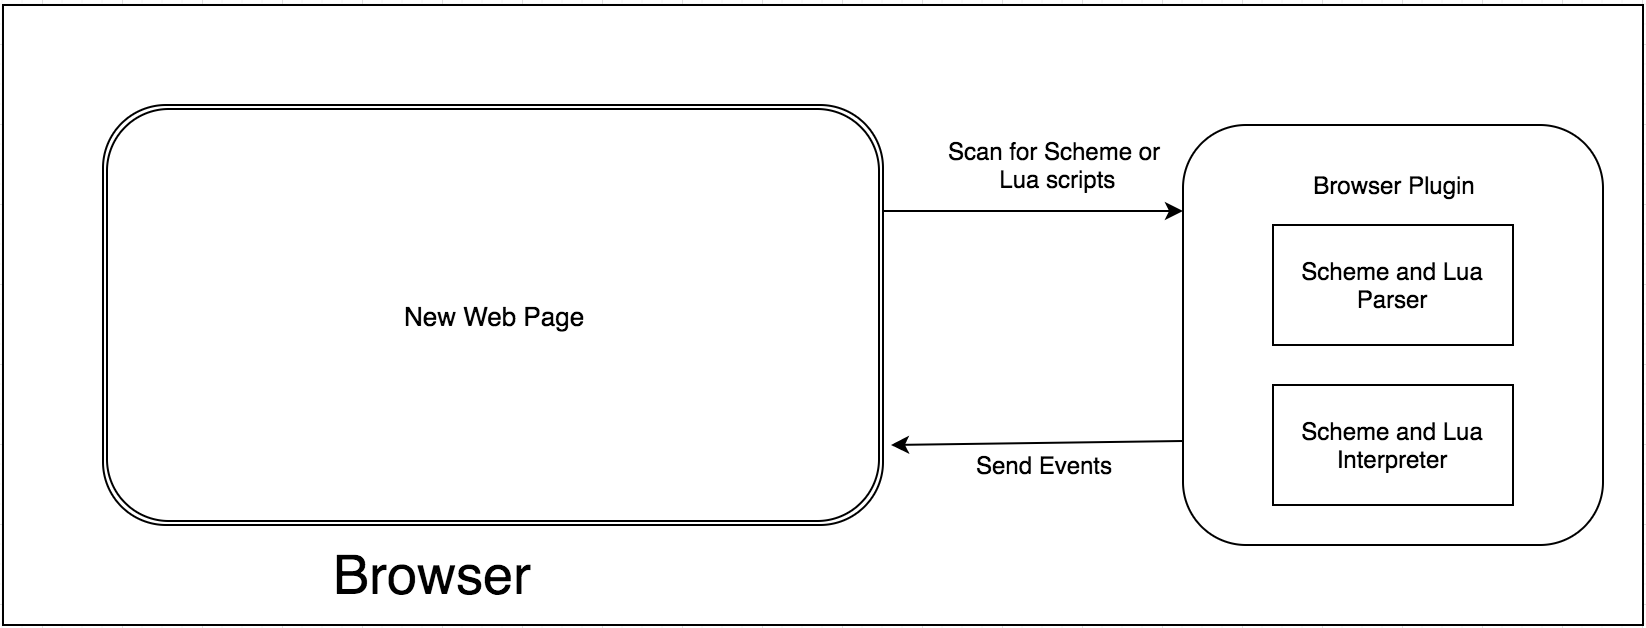
\includegraphics[width=\linewidth]{./images/browserPluginApproach.png}
	\end{center}
	\caption{Browser Plugin Approach : Architecture}
	\label{fig:pluginarchitecture}
\end{figure}

  For this approach, multi language support will be integrated into web browsers (Mozilla, Chrome) using Mozilla, and Chrome Plugin. Plugin will process, interpret any Scheme and Lua script on the page and will inject necessary event into the page again. as shown in figure \ref{fig:pluginarchitecture}
	 
  Whenever new web page is loaded into the browser, browser plugin will scan the web page for any Scheme or Lua scripts on that page. matching scripts will then be parsed by the parser and interpreter will interpret this parsed input into necessary DOM events and sends these events to the web page. 
  
  All the interaction between languages is managed by browser plugin. Advantage of having this approach is programmer does not have to worry about adding all the libraries necessary for multi language support, into the web page. Disadvantages of having this approach is, it makes interaction between these languages little complex and also, plugin needs to have permission to read scripts from the web page.
  
	
\subsection{JS Library}

\begin{figure}[ht]
	\begin{center}
		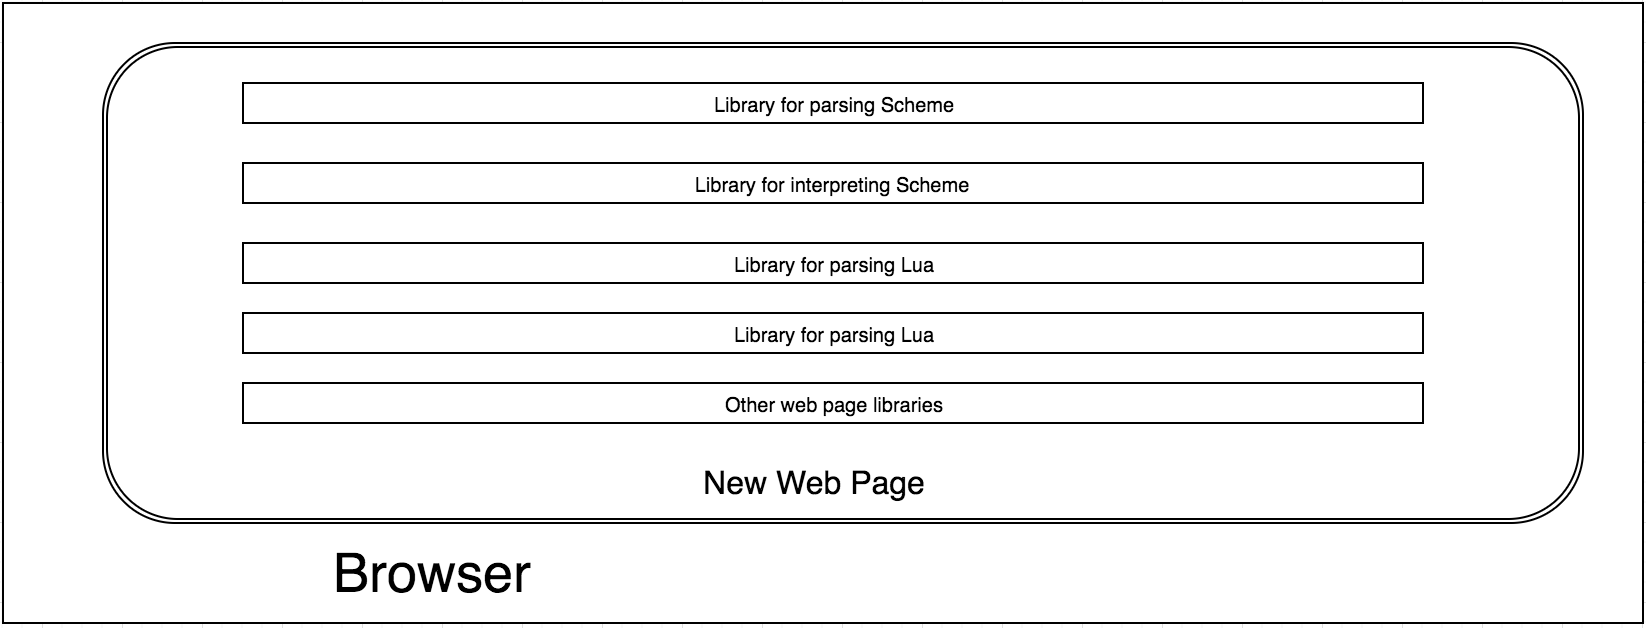
\includegraphics[width=\linewidth]{./images/JSLibraryApproach.png}
	\end{center}
	\caption{JS Library Approach : Architecture}
	\label{fig:jslibraryarchitecture}
\end{figure}

   In this approach, multi language support is achieved in web pages by including libraries in web page itself. When web page will loaded into browser, it will be loaded with necessary language support libraries, which will help browser to interpret these languages and help to achieve necessary interaction between different languages. Script can be included in browser as shown in figure \ref{fig:jslibraryarchitecture} .
   
   All the interaction between different languages is handled explicitly by the programmer by referencing these libraries in his web page directly. Advantages of taking this approach is that, programmer will get more flexibility over language interaction. Disadvantage is programmer has to take care of adding all the language specific libraries to the web page.  

\section{Challenges}

There are many challenges while building multi language support for any application. For building multi language support for browser these are some of the challenges that we came across.

\subsection{Different APIs for DOM}

To render web pages on the browser, language has to work with browser's DOM APIs. Every language has its own syntax for interacting with DOM APIs. 


Currently, there is no implementation of Scheme, and Lua for browser side platform. For this project, we had to create our own subset of Scheme, and Lua which works with browser's DOM APIs, and JavaScript. We had to write our own parser and interpreter for these languages in browser.

It was challenging to decide how the language syntax will look like for doing DOM manipulations(DOM APIs) and interacting with other languages.



\subsection{Interaction between languages}

?Section to be added.


\section{Results}

The results of this project will be, 

1) Parser and Interpreter libraries for Scheme and Lua with support for DOM and interaction with Java Script.

2) Browser plugin for Chrome, and Firefox which can execute scheme, and lua scripts from any page opened in the browser.

3) Application built using Java Script, Scheme, and Lua working together.
